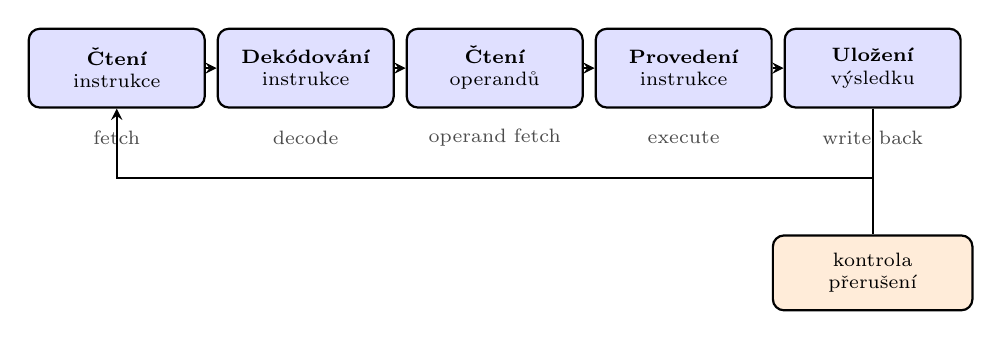
\begin{tikzpicture}[
    x=1cm, y=1cm,
    >=stealth,
    every node/.style={font=\small},
    stepbox/.style={
        draw,
        thick,
        rounded corners,
        align=center,
        text width=2.0cm,
        minimum height=1.0cm,
        minimum width=2.2cm,
        fill=blue!12
    },
    arr/.style={->, thick}
]
    % Main cycle boxes
    \node[stepbox, font=\scriptsize] (fetch) at (-4.8,0.70)
        {\textbf{Čtení}\\ instrukce};

    \node[stepbox, font=\scriptsize] (decode) at (-2.4,0.70)
        {\textbf{Dekódování}\\ instrukce};

    \node[stepbox, font=\scriptsize] (operands) at (0,0.70)
        {\textbf{Čtení}\\ operandů};

    \node[stepbox, font=\scriptsize] (execute) at (2.4,0.70)
        {\textbf{Provedení}\\ instrukce};

    \node[stepbox, font=\scriptsize] (writeback) at (4.8,0.70)
        {\textbf{Uložení}\\ výsledku};

    % Arrows between boxes
    \draw[arr] (fetch.east) -- (decode.west);
    \draw[arr] (decode.east) -- (operands.west);
    \draw[arr] (operands.east) -- (execute.west);
    \draw[arr] (execute.east) -- (writeback.west);

    % Labels under boxes
    \node[font=\scriptsize, text=gray!60!black] at (-4.8,-0.18) {fetch};
    \node[font=\scriptsize, text=gray!60!black] at (-2.4,-0.18) {decode};
    \node[font=\scriptsize, text=gray!60!black] at (0,-0.18) {operand fetch};
    \node[font=\scriptsize, text=gray!60!black] at (2.4,-0.18) {execute};
    \node[font=\scriptsize, text=gray!60!black] at (4.8,-0.18) {write back};

    % Return line
    \draw[arr]
        (writeback.south) -- (4.8,-0.7) --
        (-4.8,-0.7) -- (fetch.south);

    % Interrupt check box
    \node[
        draw,
        thick,
        rounded corners,
        fill=orange!15,
        align=center,
        text width=2.3cm,
        minimum height=0.95cm,
        font=\scriptsize
    ] (interrupt) at (4.8,-1.9)
        {kontrola\\ přerušení};

    \draw[thick] (writeback.south) -- (interrupt.north);

\end{tikzpicture}
